
%% bare_conf_compsoc.tex
%% V1.4a
%% 2014/09/17
%% by Michael Shell
%% See:
%% http://www.michaelshell.org/
%% for current contact information.
%%
%% This is a skeleton file demonstrating the use of IEEEtran.cls
%% (requires IEEEtran.cls version 1.8s or later) with an IEEE Computer
%% Society conference paper.
%%
%% Support sites:
%% http://www.michaelshell.org/tex/ieeetran/
%% http://www.ctan.org/tex-archive/macros/latex/contrib/IEEEtran/
%% and
%% http://www.ieee.org/

%%*************************************************************************
%% Legal Notice:
%% This code is offered as-is without any warranty either expressed or
%% implied; without even the implied warranty of MERCHANTABILITY or
%% FITNESS FOR A PARTICULAR PURPOSE!
%% User assumes all risk.
%% In no event shall IEEE or any contributor to this code be liable for
%% any damages or losses, including, but not limited to, incidental,
%% consequential, or any other damages, resulting from the use or misuse
%% of any information contained here.
%%
%% All comments are the opinions of their respective authors and are not
%% necessarily endorsed by the IEEE.
%%
%% This work is distributed under the LaTeX Project Public License (LPPL)
%% ( http://www.latex-project.org/ ) version 1.3, and may be freely used,
%% distributed and modified. A copy of the LPPL, version 1.3, is included
%% in the base LaTeX documentation of all distributions of LaTeX released
%% 2003/12/01 or later.
%% Retain all contribution notices and credits.
%% ** Modified files should be clearly indicated as such, including  **
%% ** renaming them and changing author support contact information. **
%%
%% File list of work: IEEEtran.cls, IEEEtran_HOWTO.pdf, bare_adv.tex,
%%                    bare_conf.tex, bare_jrnl.tex, bare_conf_compsoc.tex,
%%                    bare_jrnl_compsoc.tex, bare_jrnl_transmag.tex
%%*************************************************************************


% *** Authors should verify (and, if needed, correct) their LaTeX system  ***
% *** with the testflow diagnostic prior to trusting their LaTeX platform ***
% *** with production work. IEEE's font choices and paper sizes can       ***
% *** trigger bugs that do not appear when using other class files.       ***                          ***
% The testflow support page is at:
% http://www.michaelshell.org/tex/testflow/



\documentclass[conference]{IEEEtran}
\usepackage{savesym}
\usepackage{amsmath}
\savesymbol{iint}
\usepackage{txfonts}
\usepackage{graphicx}
%\usepackage{amssymb}
%\usepackage{verbatim}
\usepackage{algorithm} %format of the algorithm
\usepackage{algorithmic}
\usepackage{subfigure}
\usepackage{multirow}
\usepackage{epstopdf}
\usepackage{geometry}
\geometry{left=1.2cm, right=1.2cm, top=1.5cm, bottom=1.5cm}


%\let\oldforeign@language\foreign@language
%\DeclareRobustCommand{\foreign@language}[1]{%
%  \lowercase{\oldforeign@language{#1}}}
\newtheorem{definition}{\textbf{Definition}}
\newtheorem{lemma}{\textbf{Lemma}}
\newtheorem{property}{\textbf{Property}}
\newtheorem{proof}{Proof}
\newtheorem{problem}{\textbf{Problem}}



\hyphenpenalty=7000

% Some/most Computer Society conferences require the compsoc mode option,
% but others may want the standard conference format.
%
% If IEEEtran.cls has not been installed into the LaTeX system files,
% manually specify the path to it like:
% \documentclass[conference,compsoc]{../sty/IEEEtran}





% Some very useful LaTeX packages include:
% (uncomment the ones you want to load)


% *** MISC UTILITY PACKAGES ***
%
%\usepackage{ifpdf}
% Heiko Oberdiek's ifpdf.sty is very useful if you need conditional
% compilation based on whether the output is pdf or dvi.
% usage:
% \ifpdf
%   % pdf code
% \else
%   % dvi code
% \fi
% The latest version of ifpdf.sty can be obtained from:
% http://www.ctan.org/tex-archive/macros/latex/contrib/oberdiek/
% Also, note that IEEEtran.cls V1.7 and later provides a builtin
% \ifCLASSINFOpdf conditional that works the same way.
% When switching from latex to pdflatex and vice-versa, the compiler may
% have to be run twice to clear warning/error messages.






% *** CITATION PACKAGES ***
%
\ifCLASSOPTIONcompsoc
  % IEEE Computer Society needs nocompress option
  % requires cite.sty v4.0 or later (November 2003)
  \usepackage[nocompress]{cite}
\else
  % normal IEEE
  \usepackage{cite}
\fi
% cite.sty was written by Donald Arseneau
% V1.6 and later of IEEEtran pre-defines the format of the cite.sty package
% \cite{} output to follow that of IEEE. Loading the cite package will
% result in citation numbers being automatically sorted and properly
% "compressed/ranged". e.g., [1], [9], [2], [7], [5], [6] without using
% cite.sty will become [1], [2], [5]--[7], [9] using cite.sty. cite.sty's
% \cite will automatically add leading space, if needed. Use cite.sty's
% noadjust option (cite.sty V3.8 and later) if you want to turn this off
% such as if a citation ever needs to be enclosed in parenthesis.
% cite.sty is already installed on most LaTeX systems. Be sure and use
% version 5.0 (2009-03-20) and later if using hyperref.sty.
% The latest version can be obtained at:
% http://www.ctan.org/tex-archive/macros/latex/contrib/cite/
% The documentation is contained in the cite.sty file itself.
%
% Note that some packages require special options to format as the Computer
% Society requires. In particular, Computer Society  papers do not use
% compressed citation ranges as is done in typical IEEE papers
% (e.g., [1]-[4]). Instead, they list every citation separately in order
% (e.g., [1], [2], [3], [4]). To get the latter we need to load the cite
% package with the nocompress option which is supported by cite.sty v4.0
% and later.





% *** GRAPHICS RELATED PACKAGES ***
%
\ifCLASSINFOpdf
  % \usepackage[pdftex]{graphicx}
  % declare the path(s) where your graphic files are
  % \graphicspath{{../pdf/}{../jpeg/}}
  % and their extensions so you won't have to specify these with
  % every instance of \includegraphics
  % \DeclareGraphicsExtensions{.pdf,.jpeg,.png}
\else
  % or other class option (dvipsone, dvipdf, if not using dvips). graphicx
  % will default to the driver specified in the system graphics.cfg if no
  % driver is specified.
  % \usepackage[dvips]{graphicx}
  % declare the path(s) where your graphic files are
  % \graphicspath{{../eps/}}
  % and their extensions so you won't have to specify these with
  % every instance of \includegraphics
  % \DeclareGraphicsExtensions{.eps}
\fi
% graphicx was written by David Carlisle and Sebastian Rahtz. It is
% required if you want graphics, photos, etc. graphicx.sty is already
% installed on most LaTeX systems. The latest version and documentation
% can be obtained at:
% http://www.ctan.org/tex-archive/macros/latex/required/graphics/
% Another good source of documentation is "Using Imported Graphics in
% LaTeX2e" by Keith Reckdahl which can be found at:
% http://www.ctan.org/tex-archive/info/epslatex/
%
% latex, and pdflatex in dvi mode, support graphics in encapsulated
% postscript (.eps) format. pdflatex in pdf mode supports graphics
% in .pdf, .jpeg, .png and .mps (metapost) formats. Users should ensure
% that all non-photo figures use a vector format (.eps, .pdf, .mps) and
% not a bitmapped formats (.jpeg, .png). IEEE frowns on bitmapped formats
% which can result in "jaggedy"/blurry rendering of lines and letters as
% well as large increases in file sizes.
%
% You can find documentation about the pdfTeX application at:
% http://www.tug.org/applications/pdftex





% *** MATH PACKAGES ***
%
\usepackage[cmex10]{amsmath}
% A popular package from the American Mathematical Society that provides
% many useful and powerful commands for dealing with mathematics. If using
% it, be sure to load this package with the cmex10 option to ensure that
% only type 1 fonts will utilized at all point sizes. Without this option,
% it is possible that some math symbols, particularly those within
% footnotes, will be rendered in bitmap form which will result in a
% document that can not be IEEE Xplore compliant!
%
% Also, note that the amsmath package sets \interdisplaylinepenalty to 10000
% thus preventing page breaks from occurring within multiline equations. Use:
%\interdisplaylinepenalty=2500
% after loading amsmath to restore such page breaks as IEEEtran.cls normally
% does. amsmath.sty is already installed on most LaTeX systems. The latest
% version and documentation can be obtained at:
% http://www.ctan.org/tex-archive/macros/latex/required/amslatex/math/





% *** SPECIALIZED LIST PACKAGES ***
%
%\usepackage{algorithmic}
% algorithmic.sty was written by Peter Williams and Rogerio Brito.
% This package provides an algorithmic environment fo describing algorithms.
% You can use the algorithmic environment in-text or within a figure
% environment to provide for a floating algorithm. Do NOT use the algorithm
% floating environment provided by algorithm.sty (by the same authors) or
% algorithm2e.sty (by Christophe Fiorio) as IEEE does not use dedicated
% algorithm float types and packages that provide these will not provide
% correct IEEE style captions. The latest version and documentation of
% algorithmic.sty can be obtained at:
% http://www.ctan.org/tex-archive/macros/latex/contrib/algorithms/
% There is also a support site at:
% http://algorithms.berlios.de/index.html
% Also of interest may be the (relatively newer and more customizable)
% algorithmicx.sty package by Szasz Janos:
% http://www.ctan.org/tex-archive/macros/latex/contrib/algorithmicx/




% *** ALIGNMENT PACKAGES ***
%
%\usepackage{array}
% Frank Mittelbach's and David Carlisle's array.sty patches and improves
% the standard LaTeX2e array and tabular environments to provide better
% appearance and additional user controls. As the default LaTeX2e table
% generation code is lacking to the point of almost being broken with
% respect to the quality of the end results, all users are strongly
% advised to use an enhanced (at the very least that provided by array.sty)
% set of table tools. array.sty is already installed on most systems. The
% latest version and documentation can be obtained at:
% http://www.ctan.org/tex-archive/macros/latex/required/tools/


% IEEEtran contains the IEEEeqnarray family of commands that can be used to
% generate multiline equations as well as matrices, tables, etc., of high
% quality.




% *** SUBFIGURE PACKAGES ***
%\ifCLASSOPTIONcompsoc
%  \usepackage[caption=false,font=footnotesize,labelfont=sf,textfont=sf]{subfig}
%\else
%  \usepackage[caption=false,font=footnotesize]{subfig}
%\fi
% subfig.sty, written by Steven Douglas Cochran, is the modern replacement
% for subfigure.sty, the latter of which is no longer maintained and is
% incompatible with some LaTeX packages including fixltx2e. However,
% subfig.sty requires and automatically loads Axel Sommerfeldt's caption.sty
% which will override IEEEtran.cls' handling of captions and this will result
% in non-IEEE style figure/table captions. To prevent this problem, be sure
% and invoke subfig.sty's "caption=false" package option (available since
% subfig.sty version 1.3, 2005/06/28) as this is will preserve IEEEtran.cls
% handling of captions.
% Note that the Computer Society format requires a sans serif font rather
% than the serif font used in traditional IEEE formatting and thus the need
% to invoke different subfig.sty package options depending on whether
% compsoc mode has been enabled.
%
% The latest version and documentation of subfig.sty can be obtained at:
% http://www.ctan.org/tex-archive/macros/latex/contrib/subfig/




% *** FLOAT PACKAGES ***
%
%\usepackage{fixltx2e}
% fixltx2e, the successor to the earlier fix2col.sty, was written by
% Frank Mittelbach and David Carlisle. This package corrects a few problems
% in the LaTeX2e kernel, the most notable of which is that in current
% LaTeX2e releases, the ordering of single and double column floats is not
% guaranteed to be preserved. Thus, an unpatched LaTeX2e can allow a
% single column figure to be placed prior to an earlier double column
% figure. The latest version and documentation can be found at:
% http://www.ctan.org/tex-archive/macros/latex/base/


%\usepackage{stfloats}
% stfloats.sty was written by Sigitas Tolusis. This package gives LaTeX2e
% the ability to do double column floats at the bottom of the page as well
% as the top. (e.g., "\begin{figure*}[!b]" is not normally possible in
% LaTeX2e). It also provides a command:
%\fnbelowfloat
% to enable the placement of footnotes below bottom floats (the standard
% LaTeX2e kernel puts them above bottom floats). This is an invasive package
% which rewrites many portions of the LaTeX2e float routines. It may not work
% with other packages that modify the LaTeX2e float routines. The latest
% version and documentation can be obtained at:
% http://www.ctan.org/tex-archive/macros/latex/contrib/sttools/
% Do not use the stfloats baselinefloat ability as IEEE does not allow
% \baselineskip to stretch. Authors submitting work to the IEEE should note
% that IEEE rarely uses double column equations and that authors should try
% to avoid such use. Do not be tempted to use the cuted.sty or midfloat.sty
% packages (also by Sigitas Tolusis) as IEEE does not format its papers in
% such ways.
% Do not attempt to use stfloats with fixltx2e as they are incompatible.
% Instead, use Morten Hogholm'a dblfloatfix which combines the features
% of both fixltx2e and stfloats:
%
% \usepackage{dblfloatfix}
% The latest version can be found at:
% http://www.ctan.org/tex-archive/macros/latex/contrib/dblfloatfix/




% *** PDF, URL AND HYPERLINK PACKAGES ***
%
%\usepackage{url}
% url.sty was written by Donald Arseneau. It provides better support for
% handling and breaking URLs. url.sty is already installed on most LaTeX
% systems. The latest version and documentation can be obtained at:
% http://www.ctan.org/tex-archive/macros/latex/contrib/url/
% Basically, \url{my_url_here}.




% *** Do not adjust lengths that control margins, column widths, etc. ***
% *** Do not use packages that alter fonts (such as pslatex).         ***
% There should be no need to do such things with IEEEtran.cls V1.6 and later.
% (Unless specifically asked to do so by the journal or conference you plan
% to submit to, of course. )

% correct bad hyphenation here
\hyphenation{op-tical net-works semi-conduc-tor}


\begin{document}
%
% paper title
% Titles are generally capitalized except for words such as a, an, and, as,
% at, but, by, for, in, nor, of, on, or, the, to and up, which are usually
% not capitalized unless they are the first or last word of the title.
% Linebreaks \\ can be used within to get better formatting as desired.
% Do not put math or special symbols in the title.
\title{Security-Driven Task Scheduling for Multiprocessor System-on-Chips with Performance Constraints}
%


% author names and affiliations
% use a multiple column layout for up to three different
% affiliations
%\author{\IEEEauthorblockN{Nan Wang}
%\IEEEauthorblockA{School of Information Science\\
%and Engineering, ECUST\\
%Shanghai, China, 200237\\
%Email: wangnan@ecust.edu.cn}
%\and
%\IEEEauthorblockN{Song Chen}
%\IEEEauthorblockA{School of Information Science\\
% and Technology, USTC\\
%Hefei, China, 230026\\
%Email: songch@ustc.edu.cn}
%\and
%\IEEEauthorblockN{Dongxu Jiang\\ and Yu Zhu}
%\IEEEauthorblockA{School of Information Science\\
%and Engineering, ECUST\\
%Shanghai, China, 200237}}

% conference papers do not typically use \thanks and this command
% is locked out in conference mode. If really needed, such as for
% the acknowledgment of grants, issue a \IEEEoverridecommandlockouts
% after \documentclass

% for over three affiliations, or if they all won't fit within the width
% of the page (and note that there is less available width in this regard for
% compsoc conferences compared to traditional conferences), use this
% alternative format:
%
%\author{\IEEEauthorblockN{Michael Shell\IEEEauthorrefmark{1},
%Homer Simpson\IEEEauthorrefmark{2},
%James Kirk\IEEEauthorrefmark{3},
%Montgomery Scott\IEEEauthorrefmark{3} and
%Eldon Tyrell\IEEEauthorrefmark{4}}
%\IEEEauthorblockA{\IEEEauthorrefmark{1}School of Electrical and Computer Engineering\\
%Georgia Institute of Technology,
%Atlanta, Georgia 30332--0250\\ Email: see http://www.michaelshell.org/contact.html}
%\IEEEauthorblockA{\IEEEauthorrefmark{2}Twentieth Century Fox, Springfield, USA\\
%Email: homer@thesimpsons.com}
%\IEEEauthorblockA{\IEEEauthorrefmark{3}Starfleet Academy, San Francisco, California 96678-2391\\
%Telephone: (800) 555--1212, Fax: (888) 555--1212}
%\IEEEauthorblockA{\IEEEauthorrefmark{4}Tyrell Inc., 123 Replicant Street, Los Angeles, California 90210--4321}}




% use for special paper notices
%\IEEEspecialpapernotice{(Invited Paper)}




% make the title area
\maketitle

% As a general rule, do not put math, special symbols or citations
% in the abstract
\begin{abstract}
The high penetration of third-party intellectual property (3PIP) brings a high risk of malicious inclusions and data leakage in products due to the planted hardware Trojans, and system level security constraints have recently been proposed for MPSoCs protection against hardware Trojans. However, secret communication still can be established in the context of the proposed security constraints, and thus, another type of security constraints is also introduced to fully prevent such malicious inclusions. In addition, fulfilling the security constraints incurs serious overhead of schedule length, and a two-stage performance-constrained task scheduling algorithm is then proposed to maintain most of the security constraints. In the first stage, the schedule length is iteratively reduced by assigning sets of adjacent tasks into the same core after calculating the maximum weight independent set of a graph consisting of all timing critical paths. In the second stage, tasks are assigned to proper IP vendors and  scheduled to time periods with a minimization of cores required. The experimental results show that our work reduces the schedule length of a task graph, while only a small number of security constraints are violated yes.
\end{abstract}

% Note that keywords are not normally used for peerreview papers.
\begin{IEEEkeywords}
MPSoC, hardware Trojan, security, task scheduling, system performance.
\end{IEEEkeywords}






% For peer review papers, you can put extra information on the cover
% page as needed:
% \ifCLASSOPTIONpeerreview
% \begin{center} \bfseries EDICS Category: 3-BBND \end{center}
% \fi
%
% For peerreview papers, this IEEEtran command inserts a page break and
% creates the second title. It will be ignored for other modes.
\IEEEpeerreviewmaketitle

\section{Introduction}

The increased design productivity requirements for heterogeneous Multiprocessor System-on-Chip (MPSoC) require the industry to procure and use the latest Commercial-Off-The-Shelf (COTS) electronic components to track the most cutting edge technology while reducing the manufacturing costs. However, the hardware Trojans in these COTS components present high risks of malicious inclusions and data leakage in products \cite{conference:XW}. Particularly, the growing number of mission-critical applications (e.g., finance and military) that use MPSoCs means that security is the highest priority issue, whereas the increasing integration of third-party Intellectual Property (3PIP) and the outsourcing of fabrication lead to the fact that most of the MPSoCs are not 100\% trustworthy.
%and that their security-aware design is of great importance.

Emerging security problems bring an urgent need for detecting possible hardware Trojan attacks or for muting the effects. Researchers have proposed several methods for detecting hardware Trojans, which can mainly be classified into four groups: physical inspection \cite{network:SS}, functional testing \cite{conference:MM}, built-in tests \cite{conference:KX}, and side-channel analyses \cite{article:FK}. However, it is impossible to detect all of the hardware Trojans in 3PIP cores, even with the most advanced technology.

System-level security-aware design methods have also been proposed to guard systems. Beaumont \textit{et al.} \cite{conference:MB} developed an online Trojan detection architecture that implements fragmentation, replication, and voting. Rajendran \textit{et al.} \cite{article:JR} focused on the Electronic System Level (ESL) design tools and added protection against attacks at the ESL to make it more robust. Jiang \textit{et al.} \cite{conference:KJ} proposed a novel, secure-embedded systems design framework for optimizing the runtime quality. Cui \textit{et al.} \cite{conference:XC} implemented both Trojan detection and recovery at run-time, which are essential for mission-critical applications.

Recently, a set of researchers have developed the design-for-security techniques in the context of MPSoCs \cite{article:JR3} \cite{article:CL}. Rajendren \textit{et al.} \cite{conference:JR2} incorporated security constraints into the higher level design of SoCs and proposed a scheduling method for avoiding malicious output and collusion between vendors. Building on the security constraints, researchers also began to reduce the power/area/delay overhead of the technique \cite{article:NW} \cite{conference:AS}.

%Moreover, Liu et al. \cite{article:CL} proposed the scheduling of tasks under two security constraints, including \textit{task duplication}, where each task must be duplicated by the cores from different IP vendors, and \textit{vendor diversity}, where data-dependent tasks must be executed by the cores from different vendors. This security architecture successfully mutes the risks caused by collusion between 3PIPs and malicious modifications. However, the widespread use of inter-core communication leads to a significant increase in: schedule length, the number of cores required to execute all tasks, and frequent visits to the off-chip memory, including storing data in the off-chip memory and fetching data from the off-chip memory, thereby significantly degrading the quality of the design results.% In addition, Liu et al. executed the scheduling of tasks after vendor assignment, which means that the number of cores available for each task is very limited, but this could be relieved by integrating task scheduling alongside vendor assignment.

%However, fulfilling the security constraints always incurs a significant overheads in terms of design cost, area and performance delay, and we focus on how to balance these practical factors with security-aware design in this study. Security constraints are integrated into the task scheduling process in a more practical manner by considering design cost (modeled as the numbers of IP vendors required), area constraints (modeled as the number of cores available, which is also named as resource constraints) and performance constraints (modeled as schedule length).


However, secret communications between tasks may still be established in the context of the security constraints proposed in \cite{article:JR3}-\cite{article:NW}, and another type of security constraints is introduced in this study to guard the MPSoC systems. Furthermore, fulfilling the security constraints always incurs a significant overhead of performance delay, which is sensitive to the designers, and thus, a security-driven performance-constrained task scheduling method is also developed. Firstly, an edge contraction conflict graph ($ECCG$) is constructed from a timing violated graph, which consists of all paths whose delays exceed the performance constraint, and sets of edges are contracted by iteratively calculating the maximum weight independent set of $ECCG$. Then, tasks are assigned to vendors with respect to the core minimization, and they are scheduled evenly in time periods by force-directed scheduling method \cite{article:PP}. The experimental results demonstrate the high quality of the task scheduling result in reducing both the schedule length and the number of cores integrated, while most security constraints are satisfied.

%The remainder of this paper is organized as follows. Section 2 provides the preliminaries of the system-level security constraints and describes the optimization problem. Section 3 gives the details of performance-constrained task clustering, and Section 4 presents the methods for vendor assignment and task scheduling. Section 5 shows the experimental results, and Section 6 gives the conclusions.

\section{Security Constraints and Problem Description}

%At present, industry needs to procure and use the latest COTS 3PIPs to track the most cutting-edge technology while reducing the manufacturing costs, but this brings a high risk to the systems.

\subsection{Threat Model}

%3PIP cores fall into one of the three categories: soft, firm, and hard, depending on their format when they are supplied. \textcolor{blue}{Soft IP cores are described using VHDL or Verilog, and hardware Trojans can be inserted into soft IP cores by IP vendors during IP design}.


In general, the Register Transfer-Level (RTL) files of IPs might have been imported from third party vendors, and 3PIPs procured from IP vendors are usually not 100\% trustworthy. There may be a rogue insider in a 3PIP house who may insert Trojan logic in 3PIPs coming out of the IP house, and the Trojans may modify function, deny service, or create a backdoor to leak information.% and therefore, hardware Trojan protection strategy during HLS requires attation.

Detection all of the hardware Trojans in 3PIPs is extremely difficult since there is no known golden model for 3PIPs as IP vendors usually provide source code, which may contain Trojans, and when a Trojan exists in an IP core, all the fabricated ICs will contain Trojans. A Trojan can be very well hidden during the normal functional operation of the 3PIP supplied as RTL code. An attacker may distribute few RTL codes so as to reduce Trojan footprint, and a large industrial-strength IP core can include thousands of lines of code, resulting in identifying the Trojan in an IP core to be an extremely challenging task.


%At present, industry needs to procure and use the latest Commercial-Off-The-Shelf (COTS) electronic components in order to track the most cutting edge technology while reducing the manufacturing costs. However, the hardware Trojans in these COTS components present high risks of malicious inclusions and data leakage in products \cite{conference:XW2}. In the present study, we ignore the threats posed by software Trojans and only consider the protection of applications from hardware Trojans.


%3PIPs procured from IP vendors are not 100\% trustworthy. There may be a rogue insider in a 3PIP house who may insert malicious logic in 3PIPs coming out of the IP house.

%In Trojaned hardware, the attacker may modify the function, deny service, or create a backdoor to leak confidential information, thereby allowing the task running on the malicious intellectual property (IP) core to either generate additional output and trigger Trojans in other IP cores from the same vendor, or to produce incorrect outputs \cite{article:CL}. To protect applications from these risks, most previous studies have either implemented hardware Trojan detection and prevention, or security-aware system level designs.

However, many applications such as banking and military systems have high security requirements, and detecting all hardware Trojans is impossible even though with the most cutting-edge technologies;  therefore, hardware Trojan protection strategy during high level synthesis requires attention, and several system-level design-for-security methodologies have been proposed.


\subsection{Security-Driven Constraints}
\label{subsect:sec}
The recently proposed security constraints \cite{article:JR3}-\cite{article:NW}  enable a trustworthy design, and the IPs can be purchased from different vendors without worrying about their individual secruity problems. All tasks are scheduled and bound to cores under the following two security constraints.%: \textit{task duplication} and \textit{vendor diversity}.


\subsubsection{\textbf{Security Constraint 1:} Task duplication}

The probability that the Trojans implanted by different attackers have the same trigger input is quite low, and it is virtually impossible that two cores from different vendors will output the same tampered results after the same trigger input. Thus, each task is duplicately executed on the cores from different vendors, and the outputs of these cores will be compared by a trusted component (not designed by the third party) to ensure the trustworthiness of the comparison step \cite{conference:DG}. If the comparison fails, all the dependent tasks are terminated and a security flag is raised.


\subsubsection{\textbf{Security Constraint 2}: Vendor diversity between parent and its children}

To mute the Trojan footprint, attackers always distribute Trojans in multiple IP cores and construct secret communications between IP cores to leak information, or to trigger the hibernating Trojans\cite{article:CL}. In this study, we assume that the secret communication between IP cores from the same vendor cannot be acquired by other vendors and that the attackers of different vendors plant different hardware Trojans. Therefore, data-dependent tasks are executed on the cores from different vendors to isolate the triggered hardware Trojans.


%However, the \textit{redundant execution} approaches, including voting architecture \cite{conference:MB}, dual modular redundancy (DMR) \cite{conference:DG}, and task duplication constraint, detect the hardware Trojans by comparing the outputs of cores from different vendors with the same input, and they cannot cut off these secret communications. Thus the vendor diversity constraint which forces the  is also introduced to isolate the triggered hardware Trojans from the rest of the system.

%To mute the Trojan footprint, the attacker always distributes Trojans in multiple IP cores and constructs secret communications between cores to leak information or to trigger the hibernating Trojans. In this study, we assume that the secret communication between cores from the same vendor cannot be acquired by other vendors and that the attackers of different vendors plant different hardware Trojans.












\section{Motivations and Problem Description}

\subsection{Motivation 1: Security Constraint Enhancement}


An example of task scheduling with security constraints is illustrated in Fig. \ref{fig:structure}, where the solid lines represent inter-core communications, and the communication delay is marked next to the edge. Each node has four values: $v_i$ is the $i-$th task and its duplicated task is $v'_i$; $C_j$ denotes the assigned core $j$; $m-n$ are the starting and finishing times. In this example, we assume that $C1$ and $C2$ are from the first and second IP vendors, respectively, and the execution time of each task is 10 units of time (\textit{u.t.}).
\begin{figure}[!h]
\centering
\begin{tabular}{ccc}
\hspace*{-1.5em}
\subfigure [] {
\includegraphics[width=1.35cm]{figure/tg3.pdf}\label{subfig:tg3}
} &\hspace*{-1.86em}
\subfigure [] {
\includegraphics[width=4cm]{figure/TS1.pdf}\label{subfig:ts1}
} &\hspace*{-1.86em}
\subfigure [] {
\includegraphics[width=3.9cm]{figure/TS2.pdf}\label{subfig:ts2}
}
\end{tabular}
\caption{Collusion between parent and its duplicated children. \subref{subfig:tg3} Task graph. \subref{subfig:ts1} Schedule with task duplication and vendor diversity constraints. \subref{subfig:ts2} Secret communications may be established between parent and its duplicated children.}
\label{fig:structure}
\end{figure}

With all task duplication and vendor diversity constraints satisfied, the scheduling result of Liu \textit{et al.} \cite{article:CL} is given in Fig. \ref{subfig:ts1}. $v_1$ and its duplicated children $v'_2$, $v'_3$ are bound to the same core, and secret communications between ($v_1$, $v'_2$) and ($v_1$, $v'_3$) may be established because $v'_2$ and $v'_3$ are the duplicated tasks of $v_2$ and $v_3$; thus, Trojans in $C1$ may be triggered via ($v_1$, $v'_2$) or ($v_1$, $v'_3$). Due to the same reason, Trojans in $C2$ can also be triggered via ($v'_1$, $v_2$) or ($v'_1$, $v_3$). Fig. \ref{subfig:ts2} gives all possible secret communications that may be established between tasks and their duplicated children, which are represented by the dash lines. For this reason, the following security constraint is also introduced.

\textit{\textbf{Security Constraint 3}: Vendor diversity between parent and its duplicated children:} A parent task and its duplicated children are bound to the cores from different IP vendors.

%\subsubsection{Motivation 2: Schedule Length Optimization}

\subsection{Motivation 2: Trade-off Between Schedule Length and Security}


With the task graph given in Fig. \ref{subfig:tg4}, Fig. \ref{subfig:security1} shows all of the security constraints: black lines, blue lines and red lines represent the first, second, and third types of security constraints, respectively. Suppose a task graph has $n$ nodes and $m$ edges, and the number of all security constraints (denoted as $scy$) is $n+4m$.



\begin{figure}[!h]
\centering
\begin{tabular}{ccc}
\hspace*{-1em}
\subfigure [] {
\includegraphics[width=1.4cm]{figure/tg4.pdf}\label{subfig:tg4}
} &\hspace*{-0.6em}
\subfigure [] {
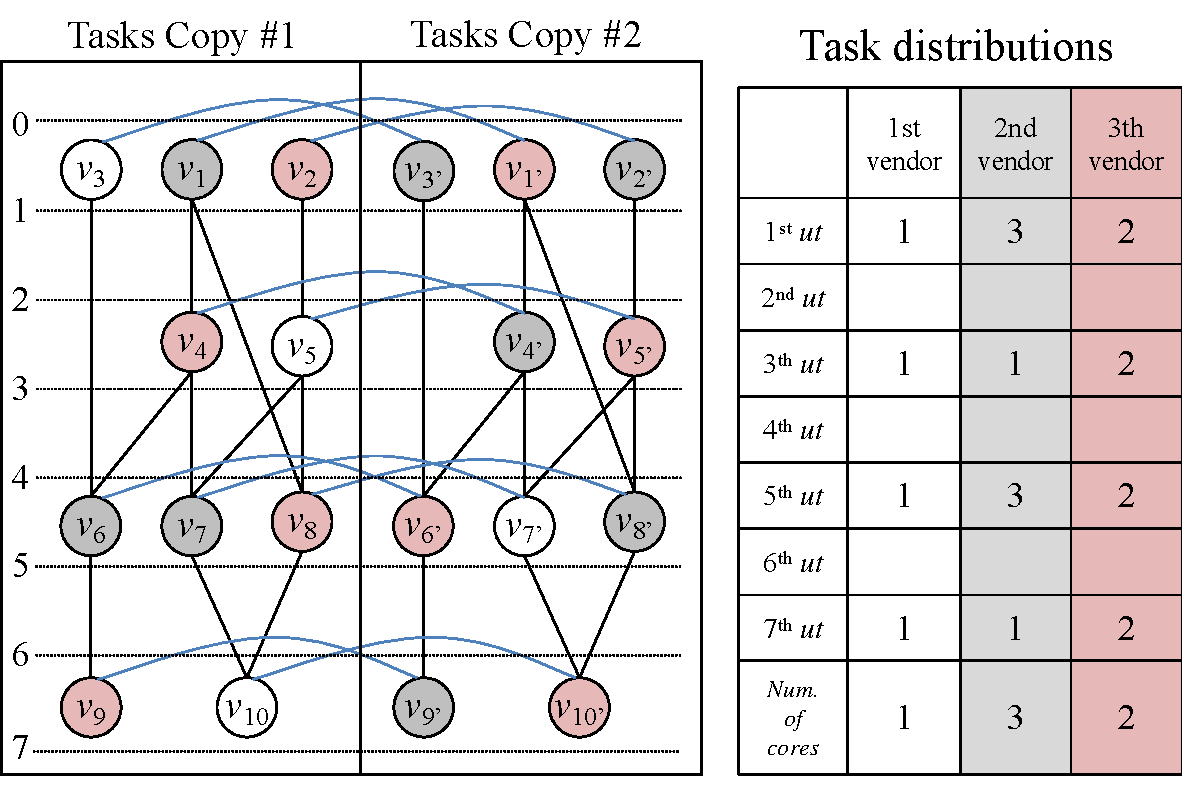
\includegraphics[width=3.3cm]{figure/security1.pdf}\label{subfig:security1}
} &\hspace*{-0.6em}
\subfigure [] {
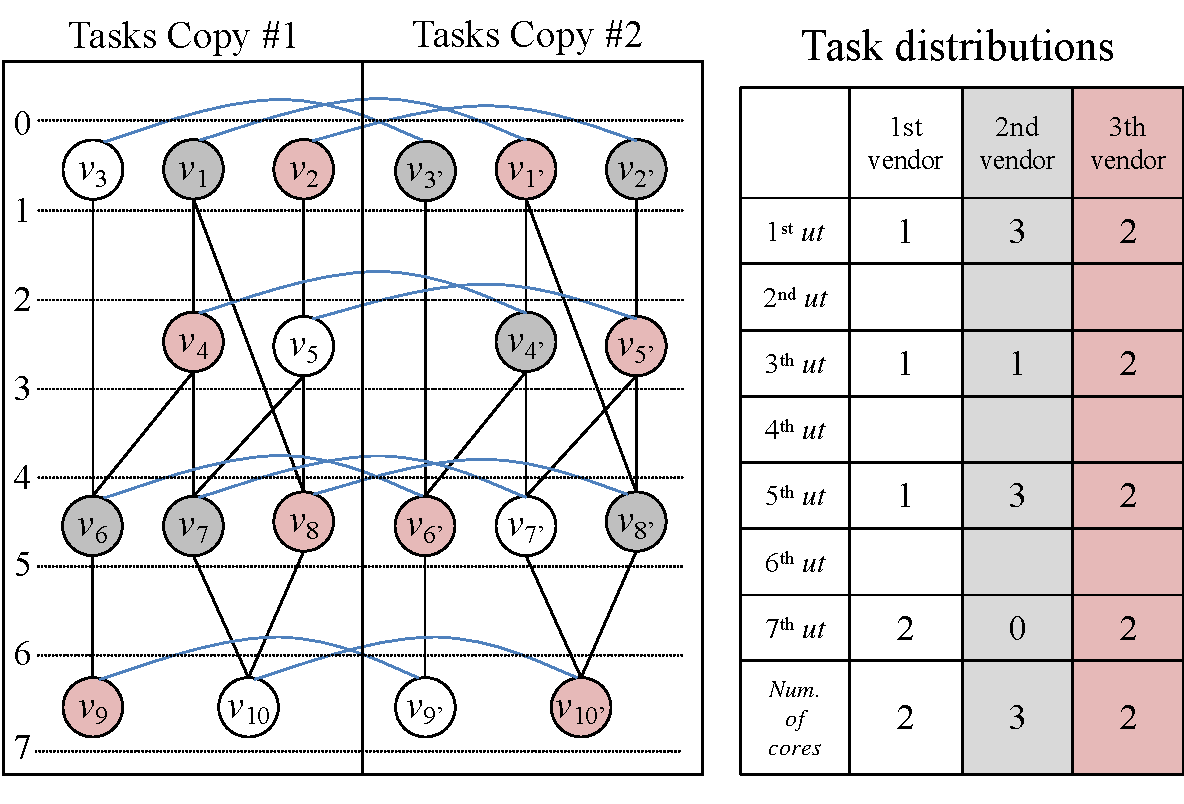
\includegraphics[width=3.3cm]{figure/security2.pdf}\label{subfig:security2}
}
\end{tabular}
\caption{Security constraints between tasks. \subref{subfig:tg4} Task graph. \subref{subfig:security1} All security constraints are satisfied. \subref{subfig:security2} Security constraints after performance optimization.}
\label{fig:security}
\end{figure}




Fulfills the security constraints at the finest granularity, but this incurs significant overhead of system performance. Therefore, researchers also explore the possibility of grouping dependent tasks into a cluster and scheduling the entire cluster to a single core to hide the inter-core communication latency \cite{article:CL} \cite{article:NW}. However, Liu \textit{et al.} \cite{article:CL} forget to minimize the Trojan triggering risk, and Wang \textit{et al.} \cite{article:NW} ignore the task criticality variation, which is also essential in evaluating the Trojan triggering risk. The edge in task graph that connects two clustered tasks is called \textit{\textbf{contracted edge}}. Task clustering violates the \textit{security constraint 2}, and the number of \textbf{\textit{security constraint violations}} is denoted as $scy_v$

The schedule length can be significantly optimized with a small number of security constraint violations. Let the inter-core communication delay be 1 $u.t.$, and the intra-core communication delay is ignored. The target is to optimize the schedule length of the task graph in Fig. \ref{subfig:tg4} by 1 $u.t.$, and the optimized result shows that only 2 out of 26 security constraints are violated if we cluster $(v_5,v_6)$ and $(v'_5,v'_6)$ (see Fig. \ref{subfig:security2}).









\subsection{Problem Description}


Let the task graph be $TG=(V,E)$, where $V$ is the set of all tasks and $E$ represents the data dependencies between tasks. The optimization problem we focused in this study is named as the security-driven performance-constrained task scheduling problem, and the performance constraint is modeled as the maximum delay that the schedule length must not exceed.

\begin{problem}
Inputs: task graph $TG$, performance constraint, and three types of security constraints. The target is to find a schedule with a minimized number of security constraint violations, and the number of cores required is also optimized.
\end{problem}

The objective function of \textit{Problem 1} is formulated as follows.
\begin{equation}
min:~\alpha*scy_v+core
\end{equation}
\noindent where $scy_v$ is the number of security constraint violations, $core$ is the number of cores required by the schedule, and $\alpha$ is a parameter large enough to keep the minimization of $scy_v$ as the first priority.

%To simplify the experiments, the core speeds of all vendors are assumed to be the same. If the core speeds of different vendors vary, this proposed method can easily be extended to fit.



%\begin{definition}[\textit{\textbf{Execution interval}}]
%The \emph{execution interval} ($EI$) of $v_i$ is defined as a consecutive time period with a length of $exec(v_i)$, where $exec(v_i)$ is the acutual execution time of $v_i$; it is denoted as $EI^{v_i}_{st}$ if its starting time is $st$. After scheduling, we write $EI^{v_i}=[s(v_i), f(v_i)]$ for simplicity.% where $s(v_i)$ and $f(v_i)$ are the starting and finishing times, respectively, of executing $v_i$.
%\end{definition}




%After assigning each task to a appropriate vendor, the real execution times of tasks can be determined, and the schedule length is calculated, which may violate the input performance constraint because we assumed that all the tasks are executed with the fastest core-speed during the task clustering stage. Let $p_c$ be the input performance constraint, $p_c'$ be the virtual performance constraint used in the task clustering stage which is initialized as $p_c$, and $sl$ be the schedule length. The principal of performing performance-constrained vendor assignment is to iteratively shorten the $p_c'$ by the schedule length overhead ($sl-p_c$) and then to execute the task clustering and vendor assignment until $sl \leq p_c$. This process is described by the pseudo codes in Algorithm \ref{alg:task_scheduling} (\textit{Lines} 2-12).



%\subsection{Performance-Constrained Task Scheduling}

%The scheduling result decides the number of cores integrated in a MPSoC and also brings significant effects to the amount of data fetched from the off-chip memory. In this work, the unit of memory ($u.m.$) is used to describe the amount of data.% Scheduling tasks evenly in each time period helps reduce the number of required cores, while maximizing the sharing of common input values in SPMs significantly reduces the amount of values fetched from the off-chip memory.



%An example of mobility derived from Fig. \ref{subfig:TG2-1} is given in Fig. \ref{subfig:mobility1}, where the computational cost of each task and the inter-core communication delay are both 10 ($u.t.$).








\section{Performance-Constrained Task Clustering}

System performance is one of the key considerations for designers, and they always put several timing-critical tasks into the same core to minimize the schedule length \cite{article:CL}. However, this brings potential risk to systems security, and thus, we must minimize the potential Trojan triggering risk when optimizing the performance.% In this section, several edges are contracted to satisfy the performance constraint; meanwhile, the number of contracted edges and the amount of data stored in the off-chip memory are simultaneously optimized.

Because $TG$ and its duplicated $TG'$ contain the same information, and contracting the data-dependent tasks into the same cluster only violates the \textit{security constraint 2}. Therefore, we only discuss the methods of contracting edges in $TG$ in the following description. Let $slack(v)$ be the slack time of $v$ under the performance constraint, and it is calculated as follows.
\begin{equation}
slack(v) = t_{alap}(v)-t_{asap}(v)-exec(v)
\end{equation}

\noindent where $exec(v)$ is the execution time of task $v$, and $t_{asap}(v)$ and $t_{alap}(v)$ are the as-soon-as-possible and as-late-as-possible schedules, respectively.% Fig. \ref{subfig:TG2} gives an example of calculating the slack time of each task in $TG$, where the virtual execution time of each task and the inter-core communication delay are both 1 ($u.t.$), and the virtual performance constraint is 5 $(u.t.)$.% The ASAP scheduling and ALAP scheduling results, and the slack times of tasks are denoted next to the tasks.% Then, the schedule length of $TG$ is iteratively reduced by contracting edges until this $TVG$ is empty.

Source and sink nodes $s$, $t$ are added to $TG$, and directed edges that pointing from $s$ to 0-indegree nodes, and from 0-outdegree nodes to $t$, are also added. An example of task graph with $s$ and $t$ is given in Fig. \ref{subfig:TG1}. Then, a \textbf{timing violated graph} $TVG=(V_T, E_T)$ is constructed, and it is an induced subgraph of $TG$. $V_T$ consists of all tasks with negative slacks, and $E_T=\{(v_i,v_j)\in E, v_i\in V_T \textrm{~and~} v_j\in V_T\}$. Let $dly(e_{ij})$ be the inter-core communication delay of $e_{ij}$, and its intra-core communication delay is ignored. Fig. \ref{subfig:tvg1-1} gives an example of $TVG$, where the performance constraint is 5 $u.t.$ and $dly(e)$ is 1 $u.t.$ for each edge.


Several edges in $TVG$ will be contracted until the performance constraint is satisfied. However, not all edges can be contracted with respect to the multi-core parallel execution. Regarding the tasks: 1) consuming the same data, or 2) feeding their computed data to the same task, they must not be assigned to the same core. This is because assigning the tasks that they once could be parallel executed to the same core forces them to be sequentially executed, which increases the schedule length of related paths. Let $in\_edge(v)$ be the set of edges that end with $v$, and $out\_edge(v)$ be the set of edges that start from $v$. Only one of the edges in $in\_edge(v)$ or $out\_edge(v)$ can be contracted.

\begin{figure}[!t]
\centering
\begin{tabular}{ccc}
\hspace*{-1.0em}
\subfigure [] {
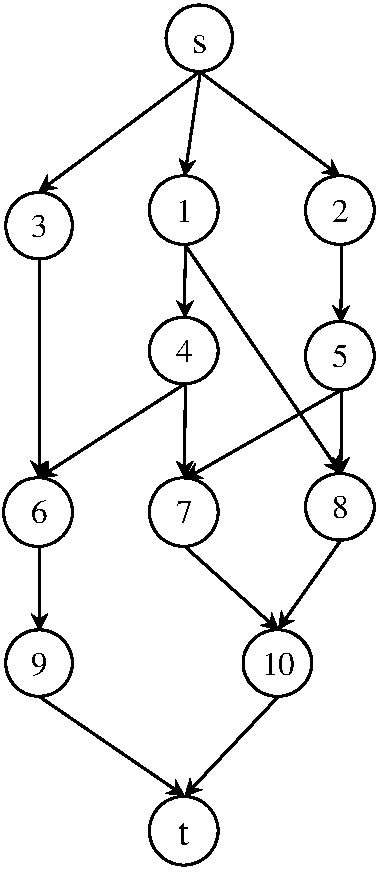
\includegraphics[width=2.33cm]{figure/TG1.pdf}\label{subfig:TG1}
}&\hspace*{-1em}
\subfigure [] {
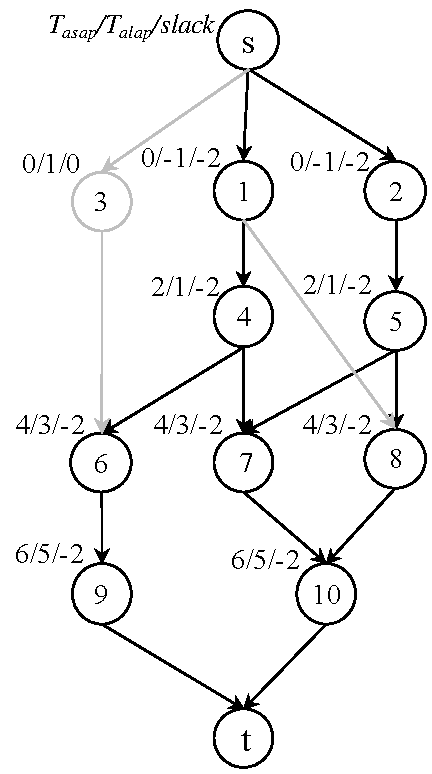
\includegraphics[width=3.02cm]{figure/tvg.pdf}\label{subfig:tvg1-1}
} &\hspace*{-1.0em}
\subfigure [] {
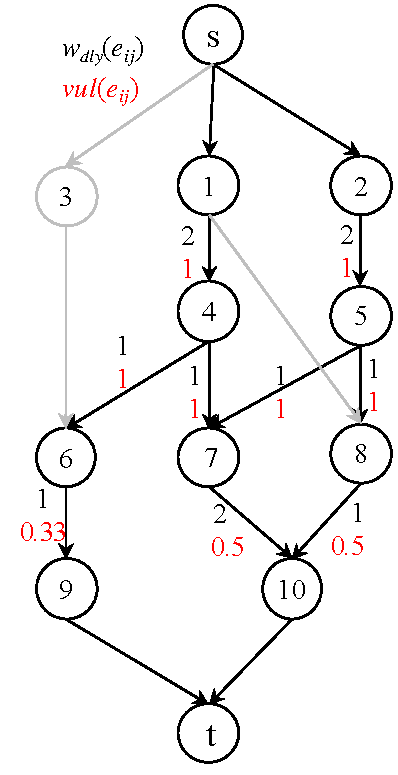
\includegraphics[width=2.85cm]{figure/tvg1.pdf}\label{subfig:tvg1-2}
}

\end{tabular}
\caption{Example of evaluating the timing violated graph. \subref{subfig:TG1} Task graph with $s$ and $t$. \subref{subfig:tvg1-1} $TVG$ with timing constraint to be 5$u.t.$ \subref{subfig:tvg1-2} The evaluation of $w_{dly}(e)$.}
\label{fig:weight_e}
\end{figure}


Contracting an edge ($e_{ij}$) with $k(u.t.)$ minimizes the lengths of all paths that passing though $e_{ij}$ by $k(u.t.)$. Let $w_{dly}(e_{ij})$ be the schedule length of $TVG$ that can be optimized after contracting $e_{ij}$, and it is estimated by the following equations.
\begin{equation}
w_{dly}(e_{ij})=\frac{path_{tvg}(e_{ij})}{path_{tvg}}*dly(e_{ij})
\end{equation}


\noindent where $path_{tvg}(e_{ij})$ is the number of paths in $TVG$ that pass through $e_{ij}$, and $path_{tvg}$ is the number of all paths in $TVG$. Fig. \ref{subfig:tvg1-2} illustrates the $w_{dly}$ in $TVG$, which is indicated next to the edge.


Clustering of timing critical tasks also necessitates information of task criticality. The total weight that evaluates these effects of contracting an edge $e_{ij}$ in $TVG$ is denoted as $w(e_{ij})$, which is calculated as follows.
\begin{equation}
w(e_{ij}) = \frac{w_{dly}(e_{ij})}{\beta*cri(v_i)}
\label{equ:weight_e}
\end{equation}

\noindent where $\beta$ is the user-determined factor, and $cri(v_i)$ is the task criticality of $v_i$.


Then, an \textbf{edge contraction conflict graph} ($ECCG$) is constructed to represent if every pair of edges can be contracted simultaneously. Set $ECCG=(V_E,E_E)$, and each vertex in $V_E$ represents an edge in $TVG$ that can be contracted. Two vertexes in $V_E$ are connected when their corresponding edges cannot be contracted simultaneously, under one of the following two situations: 1) these two edges are in the same $in\_edge(v)$ or $out\_edge(v)$ (respect to the multi-core parallel execution); 2) these two edges are in the same path (for each path in $TVG$, only one edge can be contracted in each iteration, such that the path length will not be over optimized).



\begin{figure}[!t]
\centering
\begin{tabular}{ccc}
\hspace*{-1.0em}
\subfigure [] {
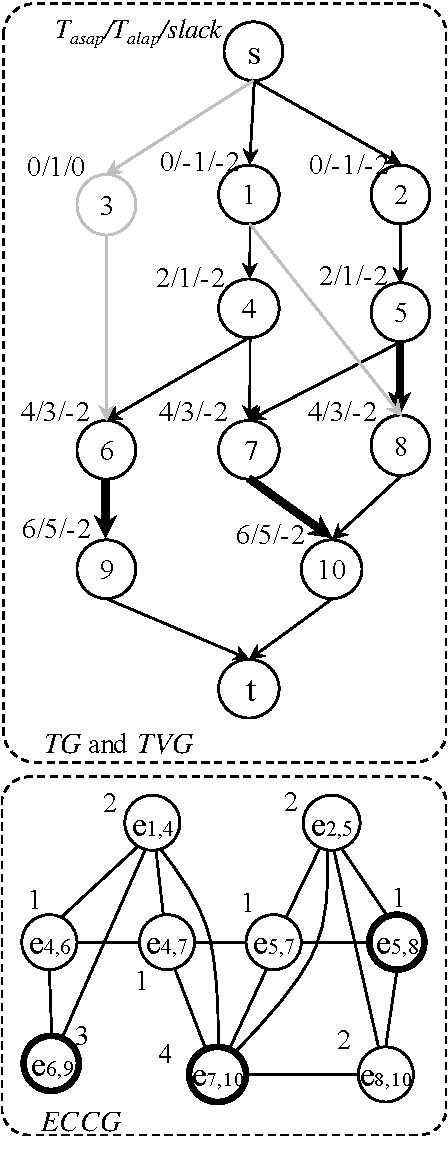
\includegraphics[width=2.93cm]{figure/EVG1.pdf}\label{subfig:EVG1}
} &\hspace*{-1.7em}
\subfigure [] {
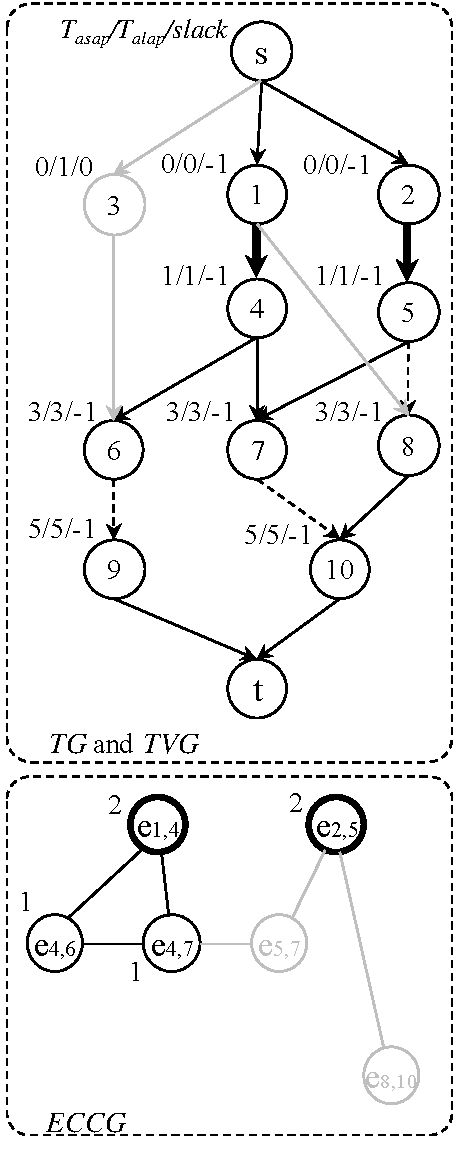
\includegraphics[width=2.93cm]{figure/EVG2.pdf}\label{subfig:EVG2}
} &\hspace*{-1.7em}
\subfigure [] {
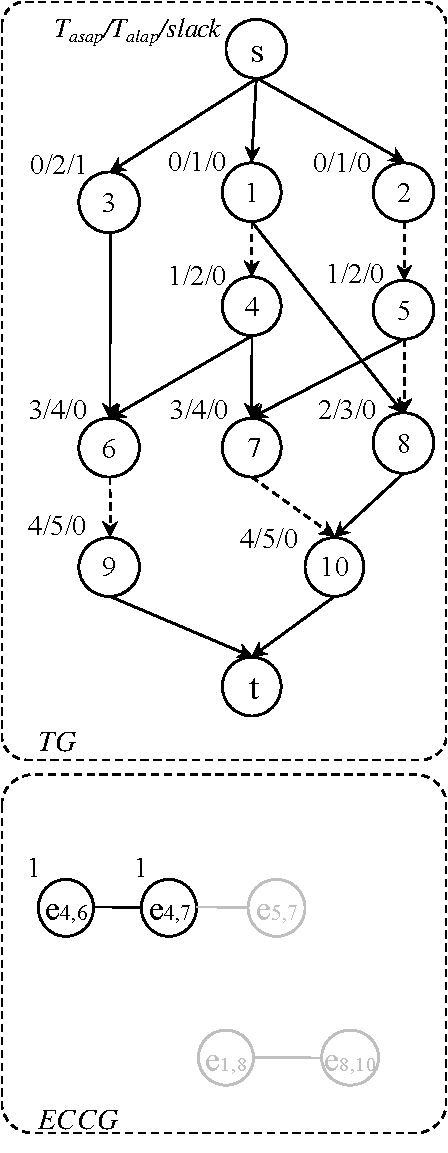
\includegraphics[width=2.9cm]{figure/EVG3.pdf}\label{subfig:EVG3}
}
\end{tabular}
\caption{Example of performance-constrained task clustering process. \subref{subfig:EVG1} The $TVG$ and its corresponding $ECCG$ before task clustering. \subref{subfig:EVG2} The $TVG$ and its corresponding $ECCG$ after the 1st iteration of task clustering. \subref{subfig:EVG3} The $TVG$ and the corresponding $VCG$ after the 2nd iteration of task clustering.}
\label{fig:TC}
\end{figure}


Clustering tasks may increase the number of IP vendors required, and if contracting an edge violate the IP vendor constraints (the method in \cite{article:NW} is applied to calculate the number IP vendors), such edge will be removed from $ECCG$. The maximum weight independent set (MWIS) of the weighted $ECCG$ is calculated by the method proposed in \cite{conference:XT}, and the set of edges in MWIS will be contracted with the maximum benefits among all possible optimization results.

An example of task clustering derived from the $TG$ in Fig. \ref{subfig:TG1} is given in Fig. \ref{fig:TC}, where we are about to optimize the schedule length by 2 $u.t.$, and the criticalities of all tasks are assumed to be the same. The $TVG$ consists of the nodes and edges with black color, and the dashed lines are the contracted edges. The $TVG$ and its corresponding $ECCG$ are first constructed (Fig. \ref{subfig:EVG1}), and its MWIS is $\{e_{1,4},~e_{2,5}\}$ which will be contracted to minimize the schedule length in the first iteration. Then, $TVG$ is updated and $ECCG$ is re-constructed as shown in Fig. \ref{subfig:EVG2}, whose MWIS is $\{e_{5,8}, e_{6,9}, e_{7,10}\}$. After contracting these edges, Fig. \ref{subfig:EVG3} gives the final clustering result.% and the corresponding $ECCG$, and $e_{5,8}$ is contracted in the final iteration.


\section{Performance-Constrained Task Scheduling}

With the task clustering results, we will decide the IP vendor assignment for each cluster, and schedule tasks to time periods to minimize the number of IP cores required. The \textbf{vendor conflict graph} ($VCG$) is constructed from the clustering results: $VCG=(V_V, E_V)$, where $V_V=\{c_1, c_2, ...\}$ is the set of clusters. An edge in $E_V$ means that the two connected clusters must be assigned to different vendors. The index of a cluster is decided by the minimum index of the tasks in this cluster. Fig. \ref{subfig:EVG3} gives an example of $VCG$ derived from the task clustering result.


\begin{definition}[Clique size]
$\omega(G)$ is the number of nodes in a \textit{maximum clique} of $G$, and it is called the \textit{clique size} of $G$.
\end{definition}

The clique size of $VCG$ equals the minimum number of vendors required, and it is calculated by the method proposed in \cite{article:NW}. The \textit{candidate vendor set} of $c_i$ comprises all of the IP vendors that can be assigned to cluster $c_i$, which is denoted as $cvs(c_i)$. The $c_i$ that can be assigned with $ipv_k$ only when

\begin{enumerate}
\item $\forall c_j \in VCG.adj\_node(c_i)$, $cvs(c_j)-ipv_k \neq \emptyset$;
\item If $v_i$ is assigned with $ipv_k$, the clique size of the new $VCG$ will not violate the vendor constraint.
\end{enumerate}


At the very beginning of vendor assignment, we assume that each cluster can be assigned with all IP vendors, and each IP vendor in \textit{candidate vendor set} has the same possibility to be assigned to the tasks in this cluster. E.g., if four IP vendors are in the $cvs(c_i)$, and the possibility of assigning $c_i$ to each IP vendor is 0.25. Then, the \textit{mobilities} of all tasks are calculated and the \textit{distribution graph} \cite{article:PP} for each IP vendor is constructed to estimate the number of cores required during vendor assignment. Let $ipv_k$ be one of the $p$ candidate vendors in $cvs(c_i)$, and $prob(v_i,t_j)$ is the probability that $v_i$ is in $t_j$. The probability that all tasks $v_m\in c_i$ are in $t_j$ and assigned to $ipv_k$ is denoted as $prob(c_i, t_j, ipv_k)$, which is calculated as follows.

\begin{equation}
prob(c_i, t_j, ipv_k)=\frac{1}{p}\sum \limits_{v_m\in c_i}prob(v_m,t_j)
\end{equation}

The next step is to take the summation of the probabilities of tasks assigned with the same vendor for each time period. The resulting distribution graph ($DG$) indicates the concurrency of tasks assigned to $ipv_k$ in $t_j$, which is calculated as follows.
\begin{equation}
DG(t_j, ipv_k) = \sum \limits_{all~clusters} prob(c_i, t_j, ipv_k)
\end{equation}

The maximum of all $DG(t_j, ipv_k), ~\forall t_j\in[1, p_c]$ is denoted as $DG_m(ipv_k)$, which is used to estimate the number of cores coming from the IP vendor $ipv_k$. The total number of cores required is denoted as $core$, and it is the sum of all estimated cores $core=\sum\limits_{\forall ipv_k}DG_m(ipv_k)$. An example of estimating the total number of cores is given in Fig. \ref{fig:ipv1}, with the clustering result demonstrated in Fig. \ref{subfig:EVG3}. Fig. \ref{subfig:vcg1} gives the $VCG$ derived from both $TG$ and $TG'$, and $c_3$ and $c_6$ are assumed to be assigned to $ipv_1$ and $ipv_3$, respectively. The mobility of each task is presented in Fig. \ref{subfig:mobility1}, and the candidate vendor set of each cluster is given in Fig. \ref{subfig:assign1}, where the number of cores required is estimated to be 7.
\begin{figure}[!t]
\centering
\begin{tabular}{cc}
\hspace*{-1.5em}
\subfigure [] {
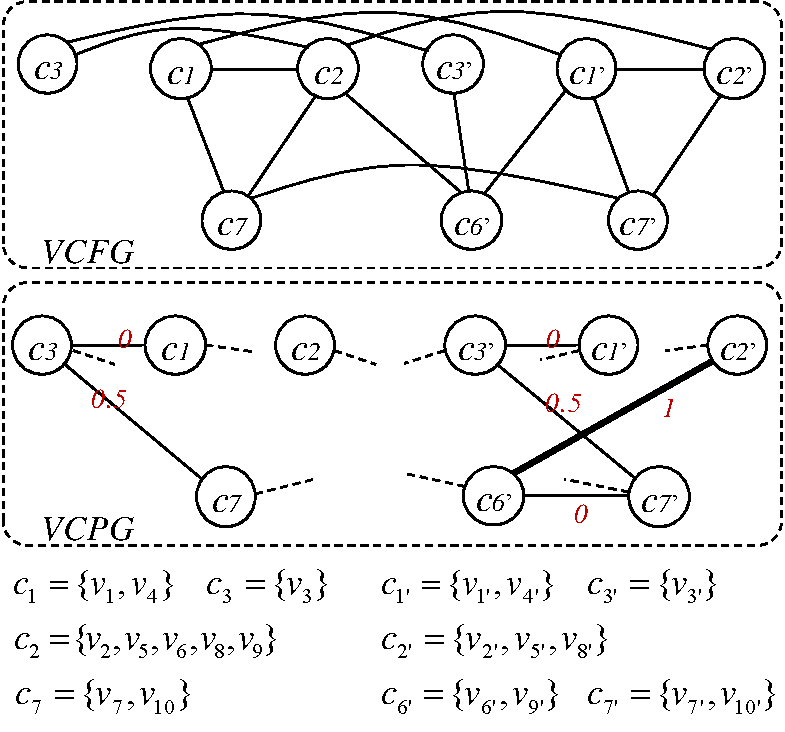
\includegraphics[width=5.5cm]{figure/vcg1.pdf}\label{subfig:vcg1}
} &\hspace*{-1em}
\subfigure [] {
\includegraphics[width=3.6cm]{figure/mobility1.pdf}\label{subfig:mobility1}
}
\end{tabular}
\begin{tabular}{c}
\hspace*{-1.5em}
\subfigure [] {
\includegraphics[width=9.7cm]{figure/dg1.pdf}\label{subfig:assign1}
}\\
\hspace*{-1.5em}
\subfigure [] {
\includegraphics[width=9.5cm, height=2.3cm]{figure/dg2.pdf}\label{subfig:assign2}
}\\
\hspace*{-1.5em}
\subfigure [] {
\includegraphics[width=9.5cm, height=2.3cm]{figure/dg3.pdf}\label{subfig:assign3}
}\\
\hspace*{-1.5em}
\subfigure [] {
\includegraphics[width=9.5cm, height=2.3cm]{figure/dg4.pdf}\label{subfig:assign4}
}
\end{tabular}
\vspace*{-0.5em}
\caption{Example of vendor assignment. \subref{subfig:vcg1} Vendor conflict graph. \subref{subfig:mobility1} The mobilities of tasks. \subref{subfig:assign1} The candidate vendor set of each cluster and the number of cores required. \subref{subfig:assign2} 7.67 cores are required if $c_1$ is assigned with $ipv_1$. \subref{subfig:assign3} 7.33 cores are required if $c_1$ is assigned with $ipv_2$. \subref{subfig:assign4} 7.33 cores are required if $c_1$ is assigned with $ipv_4$.}
\vspace*{-0.9em}
\label{fig:ipv1}
\end{figure}





To assign $c_i$ with the best IP vendor, we first estimate the number of cores required if $c_i$ is assigned to $ipv_k$, $\forall ipv_k\in cvs(c_i)$, and then assign $c_i$ to the IP vendor with the smallest number of cores required. Fig. \ref{subfig:vcg1} illustrates an example of assigning $c_1$ with proper IP vendor, where $cvs(c_1)=\{ipv_1, ipv_2, ipv_4\}$. The numbers of cores required if $c_1$ is assigned to $ipv_1$, $ipv_2$ and $ipv_4$ are 7.67, 7.33, and 7.33, respectively (see Figs. \ref{subfig:assign2} \ref{subfig:assign3} \ref{subfig:assign4}). Thus, $c_1$ will be assigned to either $ipv_2$ or $ipv_4$, because their vendor assignments are equally evaluated.



Each time after assigning a cluster with a proper IP vendor, we schedule all of the tasks in this cluster by force-directed scheduling method \cite{article:PP}. Force-directed scheduling method schedules tasks evenly in time periods, resulting in a small number of cores required. Algorithm \ref{alg:PCTC} illustrates the details of our security-Driven performance-constrained task scheduling algorithm.




\begin{algorithm}[!h]
\caption{Security-Driven Performance-Constrained Task Scheduling Algorithm, $TS(TG, p_c)$.}
\label{alg:PCTC}
\begin{algorithmic}[1]
\STATE $p_c$ is the performance constraint;
\STATE Construct $TVG$;
\WHILE{$TVG$ is not empty.}
\STATE Calculate the weight of each edge in $TVG$;
\STATE Construct $ECCG$, and calculate its MWIS;
\FOR{each $v_e\in \mathrm{MWIS}$}
    \STATE Contract $e$ in $TG$;
\ENDFOR
\STATE Calculate $slack(v), \forall v\in TG$, and construct $TVG$;
\ENDWHILE
\STATE Contract the edges in $TG'$ in the same manner;
\STATE Construct $VCG$, calculate the mobilities of all tasks, and initialize the \textit{candidate vendor sets} of all clusters.
\FOR{each un-assigned cluster $c_i$}
    \STATE Assign $c_i$ with the most suitable IP vendor $ipv_k\in cvs(c_i)$;
    \STATE Schedule all tasks in $c_i$ by force-directed scheduling \cite{article:PP}, and update the mobilities;
    \STATE Update $cvs(c_j), \forall c_j \in VCG.adj\_nodes(c_i)$;
\ENDFOR
\end{algorithmic}
\end{algorithm}


\section{Experimental Results}

\subsection{Experimental Setups}
All of the experiments were implemented in C on a Linux Workstation with an E5 2.6-GHz CPU and 32-GB RAM. To demonstrate the effectiveness of our proposed algorithms, we tested eight benchmarks from two sources\footnote{http://www.kasahara.elec.waseda.ac.jp/schedule/index.html.}: task graphs that are modeled from actual application programs, including Robot control (robot), Sparse matrix solver (sparse), SPEC fpppp (fpppp); task graphs that are randomly generagted (rnc500, rnc1000, rnc2000, rnc3000, and rnc5000). The \textit{communication-to-computation ratio} ($CCR$) is the ratio of the inter-core communication delay to the computational cost of the task, and the intra-core communication is ignored in the experiments.


%To demonstrate the effectiveness of our proposed methods, the task scheduling results of our methods are compared with a Baseline method \cite{article:CL} which schedules task strictly following the security constraints.

\subsection{Number of Vendors Required}
In this study, the third type of security constraints is introduced to enhance the system protection, and this impacts the number of vendors required. In this subsection, the numbers of vendors required are compared between the straight forward method \cite{article:CL}, and our proposed method. In the straight forward method, only the first two types of security constraints described in Sect \ref{subsect:sec} are counted, while our method uses all three types of security constraints. The number of IP vendors required is calculated by the method proposed in \cite{article:CL}.% with all three types of security constraints is tested to demonstrate the affection to the number of IP vendors.

We tested 100 task graphs that are randomly generated, and the numbers of tasks in these task graphs range from 100 to 200000. The comparison results are illustrated in Fig. \ref{fig:IP_vendor}, where $\omega(TG)$ is the clique size of task graph. The results indicate that the number of IP vendors required equals the clique size of task graph if we only follow the first two security constraints. However, if our proposed \textit{security constraint 3} is also followed, the number of IP vendors increases to four if $\omega(TG)<4$. As to the task graphs whose clique sizes are no smaller than 4, our proposed security constraints will not increase the number of vendors required.

\begin{figure}[!t]
\centering
\hspace{-0.5em}
\includegraphics[width=8.6cm,height=3.8cm]{figure/1-25.eps}
\caption{Number of IP vendors required.}
\vspace{-0.5em}
\label{fig:IP_vendor}
\end{figure}


\subsection{Performance-Constrained Task Clustering Results}


The IP vendor constraint is set to be 4 for all benchmarks, and all three types of security constraints are counted in the following experiments. Table I gives the task clustering results. The cluster-based method (\textit{Cluster}) proposed in \cite{article:CL} clusters the tasks in critical paths to optimize the schedule length, however, this method does not minimize the number of security constraint violations. Our proposed task clustering method tries to maintain a high security level when optimizing the system performance. Task criticalities for all tasks are first assumed to be the same, and thus, maximizing the security is equivalent to minimizing the $scy_v$; its clustering results are given in column $TC_1$. Then, the task criticality of $v_i$ is assumed to be the distance between $s$ and $v_i$, because the computational results may contain more confidential information when the application proceeds, and the damage to the system is also much more serious. Its corresponding clustering results are given in column $TC_2$.



\begin{table}[!h]
\renewcommand{\arraystretch}{1}
\caption{Comparisons of Performance-Constrained Task Clustering Results.}
\centering
\begin{tabular}{c|c|c|c|c|c|c|c|c|c}
\hline
\hline
task    &\multicolumn{1}{c|}{\multirow{2}{*}{$scy$}}                          &SL           &$P_c$        & \multicolumn{2}{c|}{\textit{Cluster} \cite{article:CL}}        &\multicolumn{2}{c|}{$TC_1$}   &\multicolumn{2}{c}{$TC_2$}        \\  \cline{5-6} \cline{7-8} \cline{9-10}
graph   &                                                 &\hspace*{-1em}($u.t.$)\hspace*{-1em}         &($u.t.$)       &$scy_v$     & \%  &$scy_v$     & \%   &$scy_v$     & \%    \\

\hline
\hline

\multicolumn{1}{c|}{\multirow{2}{*}{robot}}         & \multicolumn{1}{c|}{\multirow{2}{*}{612}}      &\multicolumn{1}{c|}{\multirow{2}{*}{\hspace*{-0.5em}1114\hspace*{-0.5em}}}      &997  &10     &1.63   &6   &0.98   &6   &0.98     \\
   &    &  &892   &24  &3.92  &16   &2.61    &18  &2.94 \\

\hline
\multicolumn{1}{c|}{\multirow{2}{*}{sparse}}          &\multicolumn{1}{c|}{\multirow{2}{*}{364}}     &\multicolumn{1}{c|}{\multirow{2}{*}{236}}        &208  &4  &1.10   &2   &0.55    &2   &0.55   \\
   & &    &192   &6  &1.65  &4   &1.10  &4    &1.10  \\

\hline
\multicolumn{1}{c|}{\multirow{2}{*}{fpppp}}          &\multicolumn{1}{c|}{\multirow{2}{*}{4914}}   &\multicolumn{1}{c|}{\multirow{2}{*}{\hspace*{-0.5em}2119\hspace*{-0.5em}}}  &\hspace*{-0.5em}1871\hspace*{-0.5em}  &6 &0.12  &2   &0.04  &2   &0.04  \\
   &    &   &\hspace*{-0.5em}1623\hspace*{-0.5em}   &8 &0.16   &4   &0.08  &4  &0.08 \\

\hline
\multicolumn{1}{c|}{\multirow{2}{*}{\hspace*{-0.5em}rnc500\hspace*{-0.5em}}}        &\multicolumn{1}{c|}{\multirow{2}{*}{8140}}     &\multicolumn{1}{c|}{\multirow{2}{*}{373}}    &340   &6  &0.07  &4  &0.05   &4  &0.05   \\
  &   &  &300  &26  &0.32  &18   &0.22  &22  &0.27 \\

\hline
\multicolumn{1}{c|}{\multirow{2}{*}{\hspace*{-1em}rnc1000\hspace*{-1em}}}         &\multicolumn{1}{c|}{\multirow{2}{*}{\hspace*{-1em}13020\hspace*{-1em}}}     &\multicolumn{1}{c|}{\multirow{2}{*}{254}}   &226    &16 &0.12  &12   &0.09  &14  &0.11   \\
   &  &   &203   &86  &0.66  &62   &0.48  &68  &0.52 \\

\hline
\multicolumn{1}{c|}{\multirow{2}{*}{\hspace*{-1em}rnc2000\hspace*{-1em}}}       &\multicolumn{1}{c|}{\multirow{2}{*}{\hspace*{-1em}17720\hspace*{-1em}}}       &\multicolumn{1}{c|}{\multirow{2}{*}{268}}    &243    &14  &0.08  &8      &0.05  &10 &0.06   \\
  &  &  &219   &52  &0.29  &38      &0.21  &42 &0.24  \\


\hline
\multicolumn{1}{c|}{\multirow{2}{*}{\hspace*{-1em}rnc3000\hspace*{-1em}}}        &\multicolumn{1}{c|}{\multirow{2}{*}{\hspace*{-1em}38464\hspace*{-1em}}}     &\multicolumn{1}{c|}{\multirow{2}{*}{304}}  &274  &14  &0.04  &12   &0.03   &14   &0.04  \\
   &   &  &243   &98  &0.26   &82 &0.21   &88  &0.23 \\


\hline
\multicolumn{1}{c|}{\multirow{2}{*}{\hspace*{-1em}rnc5000\hspace*{-1em}}}        &\multicolumn{1}{c|}{\multirow{2}{*}{\hspace*{-1em}64716\hspace*{-1em}}}    &\multicolumn{1}{c|}{\multirow{2}{*}{214}}    &194  &16  &0.03  &10  &0.02 &12  &0.02    \\
   &   &  &171   &92   &0.14   &74   &0.11   &80  &0.12  \\
\hline

avg.   &   &  &    &    &0.66   &    &0.42   &   &0.46  \\
\hline
\hline
\end{tabular}
\label{table:VPCTC}
\end{table}




\begin{table*}[!t]
\renewcommand{\arraystretch}{1}
\caption{Comparisons of Performance-Constrained Task Scheduling Results.}
\centering
\begin{tabular}{c|c|c|c|c|c|c|c|c|c|c|c|c|c|c|c}
\hline
\hline
task            &\multicolumn{1}{c|}{\multirow{2}{*}{tasks}}     &\multicolumn{1}{c|}{\multirow{2}{*}{$scy$}}                     &\multicolumn{1}{c|}{\multirow{2}{*}{$CCR$}}     &SL    & $P_c$              &\multicolumn{4}{c|}{\textit{Cluster} \cite{article:CL}}          &\multicolumn{4}{c|}{\textit{TS}}  &\multicolumn{2}{c}{Savings}   \\ \cline{7-10} \cline{11-14} \cline{15-16}
graph          &   &    &   &($u.t.$)   &($u.t.$)    &\multicolumn{1}{c|}{\multirow{1}{*}{$scy_v$}} &ratio (\%)    &$core$ &runtime ($s$)   &$scy_v$       &ratio (\%)  &$core$        &runtime ($s$)  &$scy_v~(\%)$   &$core~(\%)$  \\

\hline
\hline

\multicolumn{1}{c|}{\multirow{2}{*}{robot}}   &\multicolumn{1}{c|}{\multirow{2}{*}{88}}   &\multicolumn{1}{c|}{\multirow{2}{*}{612}} &0.5 &839 &671 &28   &4.58   &14  &3.4  &18   &2.94   &11   &23.5     &1.64   &21.43 \\
                                              &      &                               &1.0  &1114  &892  &24 &3.92  &14  &3.2   &16  &2.61   &10   &21.6     &1.31   &28.57  \\
\hline

\multicolumn{1}{c|}{\multirow{2}{*}{sparse}}  &\multicolumn{1}{c|}{\multirow{2}{*}{96}}  &\multicolumn{1}{c|}{\multirow{2}{*}{364}}  &0.5 &179 &143 &6  &1.65  &21  &5.1   &4   &1.10   &16    &33.8    &0.55   &23.81 \\
&  &  &1.0 &236  &189  &6   &1.65   &19   &4.8  &4   &1.10  &15  &34.7   &0.55   &21.05 \\

\hline

\multicolumn{1}{c|}{\multirow{2}{*}{fpppp}} &\multicolumn{1}{c|}{\multirow{2}{*}{334}}    &\multicolumn{1}{c|}{\multirow{2}{*}{4914}}   &0.5 &1590  &1272  &10  &0.20 &13  &7.5  &4   &0.08   &10    &57.8    &0.12   &23.08  \\
& & &1.0 &2119  &1695  &8   &0.16   &12   &7.2  &4   &0.08  &10  &58.4   &0.08   &16.67  \\

\hline

\multicolumn{1}{c|}{\multirow{2}{*}{\hspace*{-0.5em}rnc500\hspace*{-0.5em}}}   &\multicolumn{1}{c|}{\multirow{2}{*}{500}}  &\multicolumn{1}{c|}{\multirow{2}{*}{8140}}   &0.5 &280  &224  &32   &0.39   &68  &18.5  &20  &0.25   &61   &112.3    & 0.14  &10.29 \\
&  &  &1.0 &373  &300  &26   &0.32   &67   &17.2  &18 &0.22  &58   &108.9  &0.10   &13.43    \\

\hline

\multicolumn{1}{c|}{\multirow{2}{*}{\hspace*{-1em}rnc1000\hspace*{-1em}}}   &\multicolumn{1}{c|}{\multirow{2}{*}{1000}}  &\multicolumn{1}{c|}{\multirow{2}{*}{13020}}  &0.5 &190  &152  &96   &0.74  &95  &34.7 &68  &0.52   &81   &207.4    &0.22   & 14.74  \\
& & &1.0 &254  &203  &86   &0.66   &87   &36.3    &62   &0.48  &76  &203.8   &0.18   &12.64  \\

\hline

\multicolumn{1}{c|}{\multirow{2}{*}{\hspace*{-1em}rnc2000\hspace*{-1em}}}  &\multicolumn{1}{c|}{\multirow{2}{*}{2000}}  &\multicolumn{1}{c|}{\multirow{2}{*}{17720}} &0.5  &199  &159  &54   &0.31   &217   &57.3  &42   &0.24  &168   &667.5   &0.07   &22.58 \\
  & & &1.0 &268  &214  &52   &0.29   &206   &53.8   &38   &0.21  &171   &673.5   &0.08   &16.99 \\

\hline

\multicolumn{1}{c|}{\multirow{2}{*}{\hspace*{-1em}rnc3000\hspace*{-1em}}}  &\multicolumn{1}{c|}{\multirow{2}{*}{3000}}  &\multicolumn{1}{c|}{\multirow{2}{*}{38464}} &0.5 &229  &183  &106   &0.28   &238  & 158.6  &86   &0.22  &189   &1873.2   &0.06   &20.59 \\
   &  & &1.0 &304  &243  &98   &0.26   &226   &154.5   &82   &0.21   &173   &1923.3   &0.05   &23.45 \\

\hline

\multicolumn{1}{c|}{\multirow{2}{*}{\hspace*{-1em}rnc5000\hspace*{-1em}}}   &\multicolumn{1}{c|}{\multirow{2}{*}{5000}}   &\multicolumn{1}{c|}{\multirow{2}{*}{64716}} &0.5   &160  &128  &102  &0.16  &448   &278.5    &82   &0.13  &372   &2289.6   &0.03   &16.96 \\
                        &           &             &1.0                                      &214  &171  &92   &0.14   &427  &259.6  &74   &0.11   &359   &2305.7    &0.03   &15.93    \\

\hline
\multicolumn{1}{c|}{\multirow{2}{*}{avg.}}  &  & &0.5 &    &    &  &   &    &  &  &   &  &  &0.35 &19.18 \\
                                           &  &  &1.0 &     &  &   &   &    &  &  &  &  &  &0.30  &18.59 \\

\hline
\hline
\end{tabular}
\label{table:PCTS}
\end{table*}


$CCR$ is set to be 1.0, and the performance constraint $P_c$ is set as $P_c=\mathrm{\delta*SL}$, where $\mathrm{SL}$ is the schedule length with all security constraints satisfied. Two performance constraints are tested for each benchmark, with $\delta \in \{0.9, ~0.8\}$. The results show that $TC_1$ violates the minimum number of security constraints, and its $scy_v$ is reduced by 0.24\% if compared against the cluster-based method. $TC_2$ considers the task criticality variations while clustering, and its average $scy_v$ is $0.20\%$ less than that of cluster-based method.




\subsection{Performance-Constrained Task Scheduling Results}
The scheduling results of the clustered-based task scheduling method \cite{article:CL} and our proposed task scheduling method are compared in Table \ref{table:PCTS}, and columns \textit{Cluster} and \textit{TS} demonstrate their scheduling results, respectively. Two $CCRs$ (0.5 and 1.0) are tested, and the task criticality variations are ignored. The performance constraint is set to be $P_c=\mathrm{0.8*SL}$, $ratio$ is the ratio of $scy_v$ to $scy$, and $core$ is the total number of cores required by the scheduling result.

The comparison results show that, when $CCR=0.5$, our $TS$ reduces $scy_v$ by $0.35\%$ if compared against the cluster-based method; In addition, the number of cores required by our $TS$ is $19.18\%$ less than the cluster-based method. When $CCR=1.0$, our $TS$ saves $scy_v$ and $core$ by 0.30\% and 18.59\%, respectively. The runtime of our $TS$ is about 10 times larger than the cluster-based method, but the time complexities of these two methods are both $O(n^3)$, where $n$ is the number of tasks in $TG$.



%Column ``$P_c$'' gives the performance constraint that the schedule lengths of both $TG$ and $TG'$ must not exceed. In this set of experiments, we ignore the core-speed variation between vendors, and assume that 1 ($u.t.$) requires $1ms$ to execute. Each task is bound to the appropriate core following the max-cost flow-based binding algorithm \cite{conference:JC} after task scheduling. Column ``$\mathrm{FD_A}$'' gives the amount of data fetched from off-chip memory generated by the Baseline method \cite{article:CL}, and the amount of data fetched from the off-chip memory generated by our proposed method is given in column ``$\mathrm{FD_B}$''. Column ``ratio3'' gives the ratio of $\mathrm{FD_B}$ to $\mathrm{FD_A}$, and column ``runtime'' gives the runtime of vendor assignment and task scheduling (the runtime of task clustering is excluded). Column ``number of cores'' gives the number of cores required to execute all the tasks in both $TG$ and $TG'$. For the actual applications, the number of cores integrated in a MPSoC is limited; and for those randomly generated task graph whose scales are quite large, the resulting number of cores required is also large, and this can be realized by Network on Chip.

%Both the number of cores required and the amount of data fetched from off-chip memory are simultaneously optimized in the task scheduling stage, and the amount of fetched data in $\mathrm{TS_1}$ is $15.6\%$ less than $\mathrm{FD_A}$. $\mathrm{TS_2}$ equally optimizes the above two aspects, and its scheduling results further reduce the amount of fetched data by an average of 2.4\% if compared with the results of $\mathrm{TS_1}$, whereas the number of cores integrated in the MPSoC remains almost the same.


\section{Conclusions}

The security constraints introduced in this paper better protect the system from the malicious inclusions and data leakage due to the planted hardware Trojans. A design-for-security task scheduling approach is also proposed to improve the task scheduling result by reducing both the schedule length and the number of cores integrated, with only a small increase in the risk of Trojan triggering. In the first stage, the data-dependent tasks with negative slacks are iteratively clustered to reduce the schedule length until the given performance constraint is met. In the second stage, each cluster is assigned with a most proper IP vendor and tasks are scheduled by force-directed scheduling method, such that the number of cores required is minimized. The experimental results demonstrate that our proposed approach significantly minimizes the number of cores integrated in the MPSoC with performance constraint, while most of the security constraints are satisfied.



%\bibliographystyle{ieicetr}% bib style
%\bibliography{}% your bib database

\begin{thebibliography}{99}% more than 9 --> 99 / less than 10 --> 9
\bibitem{conference:XW}
X. Wang and R. Karri, ``NumChecker: detecting kernel control-flow modifying rootkits by using hardware performance counters,'' \textit{Proc. Design Automation Conference}, pp. 1-7, May 2013.

\bibitem{network:SS}
S. Swapp, \emph{Scanning Electron Microscopy (SEM)},\hskip 1em University of Wyoming.

\bibitem{conference:MM}
M. Banga and M.S. Hsiao, ``A novel sustained vector technique for the detection of hardware trojans,'' \textit{Proc. International Conference of VLSI Design}, pp. 327-332, Jan. 2009.

\bibitem{conference:KX}
K. Xiao and M. Tehranipoor, ``BISA: Built-in self-authentication for preventing hardware Trojan insertion,'' \textit{Proc. International Symposium on Hardware-Oriented Security and Trust}, pp. 45-50, 2013.

\bibitem{article:FK}
F. Koushanfar and A. Mirhoseini, ``A unified framework for multimodal submodular integrated circuits Trojan detection,'' \textit{IEEE Trans. Information Forensics and Security}, vol. 6, no. 1, pp. 162-174, Mar. 2011.

\bibitem{conference:MB}
M. Beaumont, B. Hopkins, and T. Newby, ``SAFER PATH: security architecture using fragmented execution and replication for protection against Trojaned hardware,'' \textit{Proc. Design, Automation \& Test in Europe Conference}, pp. 1000-1005, Mar. 2012.

\bibitem{article:JR}
J. Rajendran, et al., ``Belling the CAD: toward security-centric electronic system design,'' \textit{IEEE Trans. Comput.-Aided Design of Integr. Circuits and Syst.}, vol. 34, no. 11, pp. 1756-1769, Nov. 2015.

\bibitem{conference:KJ}
K. Jiang, P. Eles, and Z. Peng, ``Optimization of secure embedded systems with dynamic task sets,'' \textit{Proc. Design, Automation \& Test in Europe Conference}, pp. 1765-1770, Mar. 2013.

\bibitem{conference:XC}
X. Cui et al., ``High-level synthesis for run-time hardware Trojan detection and recovery,'' \textit{Proc. Design Automation Conference}, pp. 1-6, Jun. 2014.



\bibitem{article:JR3}
J. Rajendran, O. Sinanoglu, and R. Karri, ``Building trustworthy systems using untrusted components: a high-level synthesis approach,'', \textit{IEEE Trans. on Very Large Scale Integr. (VLSI) Syst.}, vol. 24, no. 9, pp. 2946-2959, 2016.


\bibitem{article:CL}
C. Liu, J. Rajendran, C. Yang, and R. Karri, ``Shielding heterogeneous MPSoCs from untrustworthy 3PIPs through security-driven task scheduling,'' \textit{IEEE Trans. Emerging Topics in Computing}, vol. 2, no. 4, pp. 461-472, 2014.


\bibitem{conference:JR2}
J. Rajendren, H. Zhang, O. Sinanoglu, and R. Karri, ``High-level Synthesis for Security and Trust'', \textit{Proc. International On-Line Testing Symposium}, pp. 232-233, 2013.

\bibitem{article:NW}
N. Wang, S. Chen, J. Ni, X. Ling, and Y. Zhu, ``Security-aware task scheduling using untrusted components in high-level synthesis,'' \textit{IEEE Access}, 2018, in press.


\bibitem{conference:AS}
A. Sengupta and S. Bhadauria, ``Untrusted third party digital IP cores: power-delay trade-off driven exploration of hardware Trojan secuired datapath during high level synthesis,'' \textit{Proc. Great Lakes Symposium on VLSI}, pp. 167-172, 2015.


\bibitem{article:PP}
P.G. Paulin and J.P. Knight, ``Force-directed scheduling for the behavioral synthesis of ASIC's,''  \textit{IEEE Trans. Comput. Aided-Design of Integr. Circuits and Syst.}, vol. 8, no. 6, pp. 661-679, Jun. 1989.


\bibitem{conference:DG}
D. Gizopoulos \textit{et al.}, ``Architectures for online error detection and recovery in multicore processors,'' \textit{Proc. Design, Automation and Test in Europe Conference}, pp. 533-538, Apr. 2011.


\bibitem{conference:XT}
X. Tang, H. Zhou, and P. Banerjee,  ``Leakage power optimization with dual-$V_{th}$ library in high-level synthesis,'' \textit{Proc. Design Automation Conference}, pp. 202-207, 2005.





\end{thebibliography}

% that's all folks
\end{document}


